\documentclass[]{exam}
\usepackage{epic,array,ecltree,url,calrsfs}
\usepackage[nointegrals]{wasysym}

%These tell TeX which packages to use.
\usepackage{array,epsfig}
\usepackage{amsmath}
\usepackage{amsfonts}
\usepackage{amssymb}
\usepackage{amsxtra}
\usepackage{amsthm}
\usepackage{mlextra} % must come after ams packages
\usepackage{mathrsfs}
\usepackage[dvipsnames]{xcolor}
\usepackage{array}
\usepackage{graphicx}
\graphicspath{ {../art/} }
\usepackage{subfig}
\usepackage{bm}
\usepackage{tikz}
\usepackage{multicol}
\usepackage{enumitem}

\newcommand{\twonode}{%
  \begingroup\normalfont
  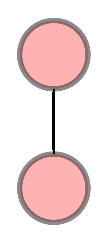
\includegraphics[height=\fontcharht\font`\b]{2nodetree.eps}%
  \endgroup
}

\newcommand{\tf}[1][{}]{%
\fillin[#1][0.25in]%
}
\title{Lab 8: Complexity, FOL, Prenex CNF}
\author{Foundations of Computer Science}
\date{\today}
%\pagestyle{empty} 
%\footer{}{\thepage}{}
\unframedsolutions
\SolutionEmphasis{\itshape\small}
\SolutionEmphasis{\color{NavyBlue}}


\begin{document}

\maketitle
\setlength{\columnseprule}{1pt}
\section*{Complexity}
\begin{questions} 
\question Recall Conway's Game of Life from the first lecture:
\url{https://bitstorm.org/gameoflife/}. Observe that as the game
progresses, each initial configuration leads inevitably to new
configurations. For example, State B in the figure below always
follows State A.
\begin{figure}[h]
\centering
\subfloat[State A]{\includegraphics{GameoflifeblinkerA.pdf}}
\qquad
\subfloat[State B]{\includegraphics{GameoflifeblinkerB.pdf}}
\end{figure}
Consider the following general problem: given two states, $A$ and $B$, you
want to determine whether starting in state $A$ will eventually lead to
state $B$. In the following questions, we refer to this problem as
$\id{con-states}$.
\begin{parts}
\part A researcher publishes a new proof that a solution to the $\id{con-states}$
problem could also be used to solve $\id{PL-SAT}$. What can we conclude
about the complexity of $\id{con-states}$?
\begin{solution}
~\\$\id{PL-SAT} \leq \id{con-states}$. $\id{PL-SAT}$ is $NP$-complete, so
$\id{con-states}$ is also $NP$-complete.
\end{solution}
\part Another researcher writes a proof showing that every instance of the
$\id{con-states}$ problem can be translated into a statement in first order
logic that is valid if and only if State $A$ eventually leads to State
$B$. What can we conclude from this (combined with the previous proof) about 
the complexity of the $\id{con-states}$ problem?
\begin{solution}
~\\$\id{con-states} \leq \id{FOL-VAL}$. $\id{FOL-VAL}$ is semi-decidable, so
$\id{con-states}$ is also semi-deciable. 
\end{solution}
\part A third proof shows that any algorithm that could determine whether
an arbitrary statement in first order logic is satisfiable, could also
be used to determine whether State $A$ eventually leads to State $B$. Given
all three proofs, what can we say about the complexity of the $\id{con-states}$
problem?
\begin{solution}
~\\$\id{con-states} \leq \id{FOL-SAT}$. $\id{FOL-SAT}$ is neither decidable
nor semi-decidable, this gives us no new information about the complexity of
$\id{con-states}$.
\end{solution}
\part Finally, a fourth proof presents the following argument: Conway's Game
of life can simulate the behavior of an arbitrary Turing machine by
encoding the machine and its input as some configuration of the board. The proof
shows how this can be done and demonstrates that the progress of the game
under these circumstances corresponds exactly to the behavior of the machine.
Furthermore, the proof shows that under these assumptions there is a state of
the board that corresponds to a Turing machine that can make no further moves. 
Assuming this is convincingly demonstrated, and taking the
three previous proofs into account, what can we conclude
about the complexity of the $\id{con-states}$ problem?
\begin{solution}
~\\Since we can assign state $A$ to any initial state of the Turing machine and
state $B$ to a halted state, the solution to $\id{con-states}$ would allow us
to determine whether an arbitrary Turing machine halts on a given input.
Therefore, $\id{HALT} \leq \id{con-states}$. Since $\id{HALT}$ is undecidable
$\id{con-states}$ is undecidable. We know from previous results that it is
also semi-decidable.
\end{solution}
\end{parts}
\clearpage

\uplevel{\section*{First Order Logic}}
\question Find a falsifying interpretation:
\begin{parts}
\part $\forall x (A(x) \imp B(x)) \imp (\exists x A(x) \imp \forall x B(x))$
\begin{solution}
~\\Domain = $\N_0$\\
$A(x) = $ the unary relation where $x \in A$ iff $x + 1$ is even.\\
$B(x) = $ the unary relation where $x \in B$ iff $x$ is odd.\\
$A(x)$ always implies $B(x)$ so $\forall x (A(x) \imp B(x))$ is true. However,
  the existence of a number $x$ such that $x + 1$ is even does not imply all
  natural numbers are odd.
\end{solution}
\part $(\forall x A(x) \lor \exists x B(x)) \imp \forall x (A(x) \lor B(x))$
\begin{solution}
~\\Same interpretation as above. The left disjunction is always true because there
exists an odd natural number. The right is false when $x$ is even.
\end{solution}
\part $(\exists x A(x) \imp \exists x B(x)) \imp \forall x(A(x) \imp B(x))$
\begin{solution}
A ``minimal'' interpretation that falsifies this formula is:\\
$(\{1,2\},\{\{1\},\{2\}\},\{\})$\\
In this example, the unary relations are simply listed in set form.\\
Another interpretation that falsifies the formula is:
~\\Domain = $\N_0$\\
$A(x) = $ the unary relation where $x \in A$ iff $x$ is even.\\
$B(x) = $ the unary relation where $x \in B$ iff $x$ is odd.\\
Since there are even and odd natural numbers, the left implication
is always true. The right is always false, since no number is even
and odd.
\end{solution}
\end{parts}
\question\label{q:tf} For each of the following expressions, give one interpretation that
makes it true and one interpretation that makes it false.
\begin{parts}
\part $\exists x p(x) \imp \forall x p(x)$
\begin{solution}
~\\
true: $(\{1\},\{\{1\}\},\{\})$ (That is, $p(x)$ is the property of being equal
    to $1$ and the domain contains only the number $1$.\\
false: $(\{1,2\},\{\{1\}\},\{\})$
\end{solution}
\part\label{q:antisym} $\forall x \forall y ((p(x,y) \land p(y,x)) \imp q(x,y))$
\begin{solution}
~\\
true: $(\N_0,\{\leq, = \},\{\})$\\ 
false: $(\N_0,\{=, < \},\{\})$
\end{solution}
\part $\forall x \forall y (f(x,y) \imp f(y,x))$
\begin{solution}
~\\
true: $(\N_0,\{ \},\{+\}, \{\})$\\ 
false:$(\N_0,\{ \},\{\div \}, \{\})$\\
Note that $f$ is a function and there is no relation in this formula.
\end{solution}

\part $\forall x \forall y \forall z (p(x,y) \imp p(f(x,z),f(y,z)))$
\begin{solution}
~\\
true: $(\Z,\{ < \},\{+\}, \{\})$\\ 
false:$(\Z,\{ < \},\{\times \}, \{\})$
\end{solution}
\end{parts}

\question Write an interpretation to the formula in question \ref{q:tf} part \ref{q:antisym}) 
above to express the claim that the substring relation is
anti-symmetric in the domain $\Sigma^*$.
\begin{solution}
$(\Sigma^*, \{substr, = \}, \{\})$
\end{solution}

\question Transform each of the following formulas to prenex normal form:
\begin{parts}
\part $\forall x(p(x) \imp \exists y q(y))$
\begin{solution}
~\\
\begin{tabular}{ll}
\text{Original formula:} & $\forall x (p(x) \imp \exists y q(y))$\\
\text{Simplify Boolean Operators:} & $\forall x (\ngg p(x) \lor \exists y q(y))$\\
\text{Extract quantifiers:} & $\forall x \exists y (\ngg p(x) \lor q(y))$
\end{tabular}
\end{solution}
\part $\forall x \forall y (\exists z p(z) \land \exists u (q(x,u) \imp \exists v q(y,v)))$
\begin{solution}
~\\
\begin{tabular}{ll}
\text{Original formula:} & $\forall x \forall y (\exists z p(z) \land \exists u
    (q(x,u) \imp \exists v q(y,v)))$\\
\text{Simplify Boolean Operators:} & $\forall x \forall y (\exists z p(z) \land
    \exists u (\ngg q(x,u) \lor \exists v q(y,v)))$\\
\text{Extract quantifiers:} & $\forall x \forall y \exists z \exists u \exists v (p(z) \land (\ngg q(x,u) \lor q(y,v)))$
\end{tabular}
\end{solution}
\part $\exists x(\ngg \exists yp(y) \imp \exists z(q(z) \imp r(x))$
\begin{solution}
~\\
\begin{tabular}{ll}
\text{Original formula:} & $\exists x(\ngg \exists yp(y) \imp \exists z(q(z) \imp r(x))$\\
\text{Simplify Boolean Operators:} & $\exists x(\ngg \ngg \exists yp(y) \lor \exists z(\ngg q(z) \lor r(x))$\\
\text{Push negation invwards:} & $\exists x(\exists yp(y) \lor \exists z(\ngg q(z) \lor r(x))$\\
\text{Extract quantifiers:} & $\exists x \exists y \exists z (p(y) \lor \ngg q(z) \lor r(x))$\\
\end{tabular}
\end{solution}
\end{parts}

\question Suppose that we allowed the domain of an interpretation to be
$\emph{empty}$. What would this mean for the equivalence:
\[ \forall y p(y,y) \lor \exists x q(x,x) \equiv \exists x (\forall y p (y,y) \lor q(x,x))\]
\begin{solution}
~\\
From Ben Ari:\\
``A universal quantified formula $\forall xA(x)$ is true in an empty domain: it has to be true 
for all elements of the domain, but there aren’t any so it is vacuously true. An existentially 
quantified formula $\exists A(x)$ is false in an empty domain: it has to be true for some 
element of the domain, but there aren’t any so it can’t be true. The equivalence is therefore 
incorrect: the left-hand side is true because $\forall yp(y,y)$ is vacuously true, while the 
right-hand side is false because it is an existentially quantified formula and the domain is 
empty. If the domain is non-empty, the equivalence holds.''
\end{solution}

\question Recall that the ``brute force'' approach to satisfiability in
propositional logic involves enumerating all possible interpretations of a
formula, which requires $2^n$ interpretations for a formula with $n$ variables.
\begin{parts}
\part Why can't we do this for first order logic?
\begin{solution}
In propositional logic interpretations assign each atom a value from a binary
domain. In first order logic, the interpretation must first specify a domain,
which can be chosen from an infinite number of sets. In addition, the number
of $n-ary$ functions and relations that can be a assigned is a function of the size
of the chosen domain. In the case that the domain is infinite, these are also
infinite.
\end{solution}
\part Assume we restrict our attention to interpretations where the domain is
$\{1,2,3\}$. How many possible binary relations are there over this domain?  
\begin{solution}
A binary relation is a set of tuples $(x,y)$ where $x, y \in \{1,2,3\}$.
Therefore, the total number of possible relations is the number of subsets
of $\{1,2,3\} \times \{1,2,3\}$, which is $2^{3^2} = 512$.
\end{solution}
\part How many possible binary functions are there over the same domain?
\begin{solution}
A binary function is a type of binary relation, so it can also be represented
as a set of pairs. Since functions can have only one output per input, there
are at most three tuples in the set. If we assume the function is a total
function over the domain, all three input values, must be represented so
there is exactly three tuples in the set. In this case, the number of
possibilities is $3^3 = 27$ (each of the three inputs can have one of $3$
outputs). If we include partial functions, we have to add in functions that
map only $1$ value, only $2$, values, or $0$ values (i.e. the empty function).
There are $9$ functions that map only one value ($3$ possible input values
and $3$ values each they could map to) and $27$ functions that map only two
values ($3$ choices of which pairs of values to map and $3$ possible mappings
for each of the input values in the pair). Finally, there is only one empty
function, so the total number of partial functions is $64$.
\end{solution}
\part Consider the set of formulas in first order logic that are restricted to
binary relations (no constants or functions). Is there a viable brute force approach 
to the satisfiability problem when the domain is restricted to $\{1,2,3\}$? If
not, why not? If so, how many interpretations do we need to check in the worst
case?
\begin{solution}
Yes. Since there are $512$ binary relations and $3$ choices of variable
assignments for each of the $2$ input variables for each binary relation,
a brute force approach would require checking $512 \times 3^2 = 4068$ 
possibilities for a formula with a single predicate. Therefore, a formula
with $n$ predicates would require enumeration of $4068^n$ possibilities. 
\end{solution}
\part How does the above answer change if we allow binary functions (but still
    no constants)?
\begin{solution}
The answer does not change. Since we know each function must have an output
in the domain, we can ignore the interpretation assigned to the function and
just check all possible outputs of any function, which is the same as all
elements in the domain. This amounts to checking against all possible
inputs to the relations, which is equivalent to checking the same formula with
no functions in it.
\end{solution}
\end{parts}

\end{questions}
\end{document}


